\documentclass{standalone}
\usepackage{tikz}
\usetikzlibrary{patterns, positioning}


\begin{document}
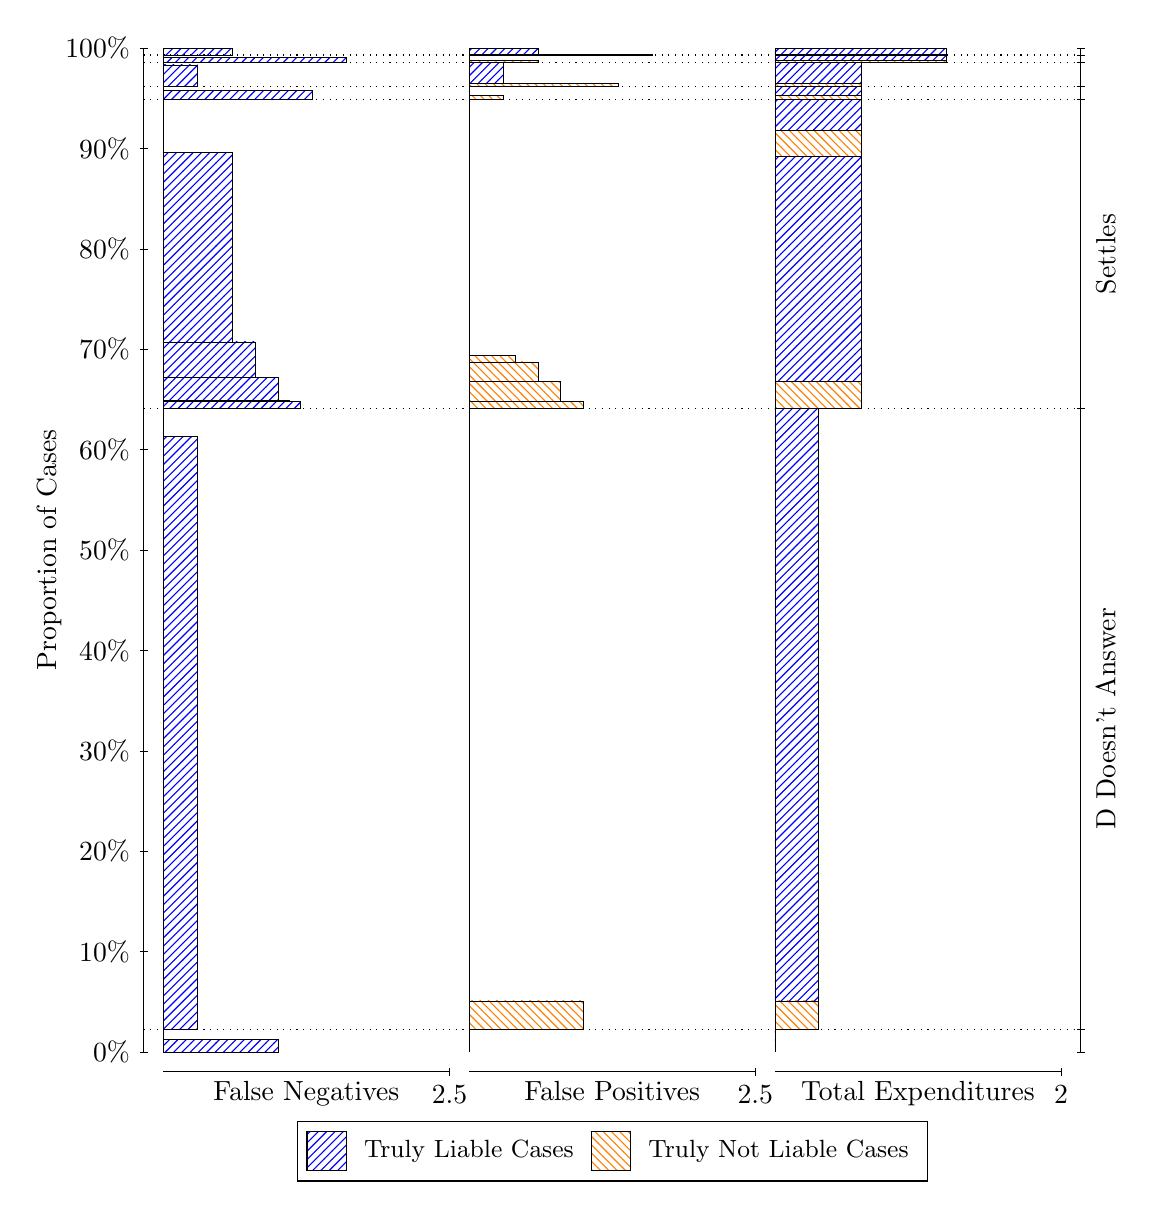
\begin{tikzpicture}
\draw[black, very thin] (1.5,1.75) -- (1.5,14.5);
\node[rotate=90, text=black, anchor=center] at (0.3, 8.125) {Proportion of Cases};
\draw[black, very thin] (1.45,1.75) -- (1.55,1.75);
\node[text=black, anchor=east] at (1.45, 1.75) {0\%};
\draw[black, very thin] (1.45,3.025) -- (1.55,3.025);
\node[text=black, anchor=east] at (1.45, 3.025) {10\%};
\draw[black, very thin] (1.45,4.3) -- (1.55,4.3);
\node[text=black, anchor=east] at (1.45, 4.3) {20\%};
\draw[black, very thin] (1.45,5.575) -- (1.55,5.575);
\node[text=black, anchor=east] at (1.45, 5.575) {30\%};
\draw[black, very thin] (1.45,6.85) -- (1.55,6.85);
\node[text=black, anchor=east] at (1.45, 6.85) {40\%};
\draw[black, very thin] (1.45,8.125) -- (1.55,8.125);
\node[text=black, anchor=east] at (1.45, 8.125) {50\%};
\draw[black, very thin] (1.45,9.4) -- (1.55,9.4);
\node[text=black, anchor=east] at (1.45, 9.4) {60\%};
\draw[black, very thin] (1.45,10.675) -- (1.55,10.675);
\node[text=black, anchor=east] at (1.45, 10.675) {70\%};
\draw[black, very thin] (1.45,11.95) -- (1.55,11.95);
\node[text=black, anchor=east] at (1.45, 11.95) {80\%};
\draw[black, very thin] (1.45,13.225) -- (1.55,13.225);
\node[text=black, anchor=east] at (1.45, 13.225) {90\%};
\draw[black, very thin] (1.45,14.5) -- (1.55,14.5);
\node[text=black, anchor=east] at (1.45, 14.5) {100\%};

\draw[black, very thin] (13.4,1.75) -- (13.4,14.5);
\draw[black, very thin] (13.35,1.75) -- (13.45,1.75);
\node[anchor=west] at (13.35, 1.75) {};
\draw[black, very thin] (13.35,2.0365) -- (13.45,2.0365);
\node[anchor=west] at (13.35, 2.0365) {};
\draw[black, very thin] (13.35,9.9268) -- (13.45,9.9268);
\node[anchor=west] at (13.35, 9.9268) {};
\draw[black, very thin] (13.35,13.843) -- (13.45,13.843);
\node[anchor=west] at (13.35, 13.843) {};
\draw[black, very thin] (13.35,14.017) -- (13.45,14.017);
\node[anchor=west] at (13.35, 14.017) {};
\draw[black, very thin] (13.35,14.318) -- (13.45,14.318);
\node[anchor=west] at (13.35, 14.318) {};
\draw[black, very thin] (13.35,14.411) -- (13.45,14.411);
\node[anchor=west] at (13.35, 14.411) {};
\draw[black, very thin] (13.35,14.5) -- (13.45,14.5);
\node[anchor=west] at (13.35, 14.5) {};

\draw[black, very thin, pattern color=blue, pattern=north east lines] (1.75,1.75) rectangle (3.2033,1.912);
\draw[black, very thin, pattern color=orange, pattern=north west lines] (1.75,1.912) rectangle (1.75,2.0365);
\draw[black, very thin, pattern color=blue, pattern=north east lines] (1.75,2.0365) rectangle (2.186,9.5645);
\draw[black, very thin, pattern color=orange, pattern=north west lines] (1.75,9.5645) rectangle (1.75,9.9268);
\draw[black, very thin, pattern color=blue, pattern=north east lines] (1.75,9.9268) rectangle (3.494,10.013);
\draw[black, very thin, pattern color=blue, pattern=north east lines] (1.75,10.013) rectangle (3.3487,10.025);
\draw[black, very thin, pattern color=blue, pattern=north east lines] (1.75,10.025) rectangle (3.2033,10.316);
\draw[black, very thin, pattern color=blue, pattern=north east lines] (1.75,10.316) rectangle (2.9127,10.769);
\draw[black, very thin, pattern color=blue, pattern=north east lines] (1.75,10.769) rectangle (2.622,13.175);
\draw[black, very thin, pattern color=orange, pattern=north west lines] (1.75,13.175) rectangle (1.75,13.843);
\draw[black, very thin, pattern color=blue, pattern=north east lines] (1.75,13.843) rectangle (3.6393,13.963);
\draw[black, very thin, pattern color=orange, pattern=north west lines] (1.75,13.963) rectangle (1.75,14.017);
\draw[black, very thin, pattern color=blue, pattern=north east lines] (1.75,14.017) rectangle (2.186,14.286);
\draw[black, very thin, pattern color=orange, pattern=north west lines] (1.75,14.286) rectangle (1.75,14.318);
\draw[black, very thin, pattern color=blue, pattern=north east lines] (1.75,14.318) rectangle (4.0753,14.386);
\draw[black, very thin, pattern color=orange, pattern=north west lines] (1.75,14.386) rectangle (1.75,14.411);
\draw[black, very thin, pattern color=blue, pattern=north east lines] (1.75,14.411) rectangle (2.622,14.493);
\draw[black, very thin, pattern color=orange, pattern=north west lines] (1.75,14.493) rectangle (1.75,14.5);
\draw[black, very thin, pattern color=orange, pattern=north west lines] (5.6333,1.75) rectangle (5.6333,1.8745);
\draw[black, very thin, pattern color=blue, pattern=north east lines] (5.6333,1.8745) rectangle (5.6333,2.0365);
\draw[black, very thin, pattern color=orange, pattern=north west lines] (5.6333,2.0365) rectangle (7.0867,2.3988);
\draw[black, very thin, pattern color=blue, pattern=north east lines] (5.6333,2.3988) rectangle (5.6333,9.9268);
\draw[black, very thin, pattern color=orange, pattern=north west lines] (5.6333,9.9268) rectangle (7.0867,10.015);
\draw[black, very thin, pattern color=orange, pattern=north west lines] (5.6333,10.015) rectangle (6.796,10.269);
\draw[black, very thin, pattern color=orange, pattern=north west lines] (5.6333,10.269) rectangle (6.5053,10.507);
\draw[black, very thin, pattern color=orange, pattern=north west lines] (5.6333,10.507) rectangle (6.36,10.514);
\draw[black, very thin, pattern color=orange, pattern=north west lines] (5.6333,10.514) rectangle (6.2147,10.595);
\draw[black, very thin, pattern color=blue, pattern=north east lines] (5.6333,10.595) rectangle (5.6333,13.843);
\draw[black, very thin, pattern color=orange, pattern=north west lines] (5.6333,13.843) rectangle (6.0693,13.898);
\draw[black, very thin, pattern color=blue, pattern=north east lines] (5.6333,13.898) rectangle (5.6333,14.017);
\draw[black, very thin, pattern color=orange, pattern=north west lines] (5.6333,14.017) rectangle (7.5227,14.05);
\draw[black, very thin, pattern color=blue, pattern=north east lines] (5.6333,14.05) rectangle (6.0693,14.318);
\draw[black, very thin, pattern color=orange, pattern=north west lines] (5.6333,14.318) rectangle (6.5053,14.343);
\draw[black, very thin, pattern color=blue, pattern=north east lines] (5.6333,14.343) rectangle (5.6333,14.411);
\draw[black, very thin, pattern color=orange, pattern=north west lines] (5.6333,14.411) rectangle (7.9587,14.419);
\draw[black, very thin, pattern color=blue, pattern=north east lines] (5.6333,14.419) rectangle (6.5053,14.5);
\draw[black, very thin, pattern color=orange, pattern=north west lines] (9.5167,1.75) rectangle (9.5167,1.8745);
\draw[black, very thin, pattern color=blue, pattern=north east lines] (9.5167,1.8745) rectangle (9.5167,2.0365);
\draw[black, very thin, pattern color=orange, pattern=north west lines] (9.5167,2.0365) rectangle (10.062,2.3988);
\draw[black, very thin, pattern color=blue, pattern=north east lines] (9.5167,2.3988) rectangle (10.062,9.9268);
\draw[black, very thin, pattern color=orange, pattern=north west lines] (9.5167,9.9268) rectangle (10.607,10.269);
\draw[black, very thin, pattern color=blue, pattern=north east lines] (9.5167,10.269) rectangle (10.607,13.127);
\draw[black, very thin, pattern color=orange, pattern=north west lines] (9.5167,13.127) rectangle (10.607,13.454);
\draw[black, very thin, pattern color=blue, pattern=north east lines] (9.5167,13.454) rectangle (10.607,13.843);
\draw[black, very thin, pattern color=orange, pattern=north west lines] (9.5167,13.843) rectangle (10.607,13.898);
\draw[black, very thin, pattern color=blue, pattern=north east lines] (9.5167,13.898) rectangle (10.607,14.017);
\draw[black, very thin, pattern color=orange, pattern=north west lines] (9.5167,14.017) rectangle (10.607,14.05);
\draw[black, very thin, pattern color=blue, pattern=north east lines] (9.5167,14.05) rectangle (10.607,14.318);
\draw[black, very thin, pattern color=orange, pattern=north west lines] (9.5167,14.318) rectangle (11.697,14.343);
\draw[black, very thin, pattern color=blue, pattern=north east lines] (9.5167,14.343) rectangle (11.697,14.411);
\draw[black, very thin, pattern color=orange, pattern=north west lines] (9.5167,14.411) rectangle (11.697,14.419);
\draw[black, very thin, pattern color=blue, pattern=north east lines] (9.5167,14.419) rectangle (11.697,14.5);
\draw[black, dotted] (1.5,2.0365) -- (13.4,2.0365);
\draw[black, dotted] (1.5,9.9268) -- (13.4,9.9268);
\draw[black, dotted] (1.5,13.843) -- (13.4,13.843);
\draw[black, dotted] (1.5,14.017) -- (13.4,14.017);
\draw[black, dotted] (1.5,14.318) -- (13.4,14.318);
\draw[black, dotted] (1.5,14.411) -- (13.4,14.411);
\draw[black, very thin] (1.75,1.5) -- (5.3833,1.5);
\node[text=black, anchor=north] at (3.5667, 1.5) {False Negatives};
\draw[black, very thin] (5.3833,1.45) -- (5.3833,1.55);
\node[text=black, anchor=north] at (5.3833, 1.45) {2.5};

\draw[black, very thin] (5.6333,1.5) -- (9.2667,1.5);
\node[text=black, anchor=north] at (7.45, 1.5) {False Positives};
\draw[black, very thin] (9.2667,1.45) -- (9.2667,1.55);
\node[text=black, anchor=north] at (9.2667, 1.45) {2.5};

\draw[black, very thin] (9.5167,1.5) -- (13.15,1.5);
\node[text=black, anchor=north] at (11.333, 1.5) {Total Expenditures};
\draw[black, very thin] (13.15,1.45) -- (13.15,1.55);
\node[text=black, anchor=north] at (13.15, 1.45) {2};


\node[text=black, centered, rotate=90] at (13.72, 5.9816) {D Doesn't Answer};
\node[text=black, centered, rotate=90] at (13.72, 11.885) {Settles};





\draw (7.449999999999999,1.5) node[draw=none] (baseCoordinate) {};
\begin{scope}[align=center]
        \matrix[scale=0.5, draw=black, below=0.5cm of baseCoordinate, nodes={draw}, column sep=0.1cm]{
            \node[rectangle, draw, minimum width=0.5cm, minimum height=0.5cm, pattern color=blue, pattern=north east lines] {}; &
            \node[draw=none, font=\small, text=black] (B) {Truly Liable Cases}; &
            \node[rectangle, draw, minimum width=0.5cm, minimum height=0.5cm, pattern color=orange, pattern=north west lines] {}; &
            \node[draw=none, font=\small, text=black] (B) {Truly Not Liable Cases}; \\
            };
\end{scope}

\end{tikzpicture}
\end{document}